\textbf{Dans cet exercice, les parties A et B sont indépendantes.}

\medskip

\begin{minipage}[t]{0.47\linewidth}
\subsection*{Partie A}
On a tracé ci-contre la courbe représentative de la fonction qui donne le volume d'une boule en~$\mathrm{cm}^{3}$ en fonction de son rayon en~cm.

\begin{enumerate}
	\item Déterminer graphiquement l'image de 3,6 par cette fonction.

	\item Le volume d'une boule est égal à \np[cm^3]{660}.

	Lire graphiquement son rayon.
\end{enumerate}
\end{minipage}
\hfill~
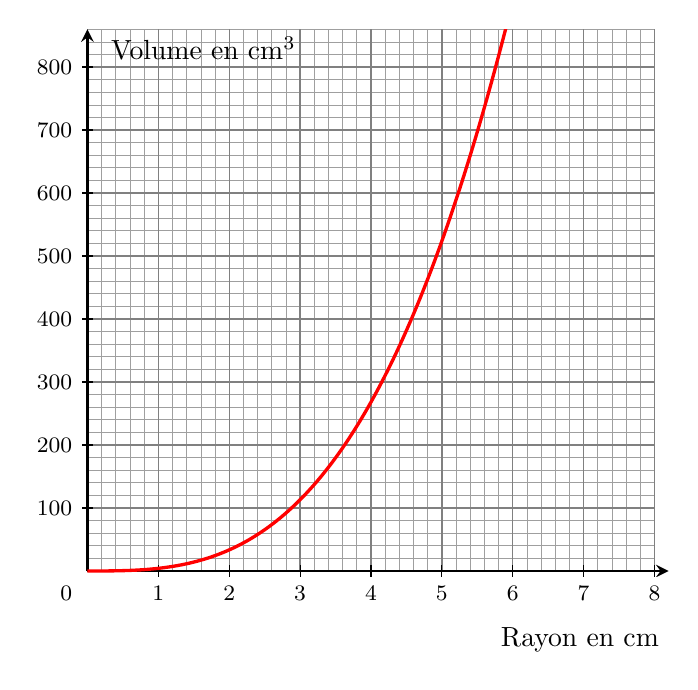
\begin{tikzpicture}[x=9mm,y=0.08mm,baseline={(vol.base)},> =stealth]
	\draw [color = gray!75, line width = 0.25pt, xstep=0.2, ystep = 20] (0,0) grid (8,860);
	\draw [color = gray, line width = 0.5pt, xstep=1, ystep = 100] (0,0) grid (8,860);
	\draw[->,line width=1pt] (0,0) -- (8.2,0);
	\node[left] at (8.2,-25pt) {Rayon en cm};
	\foreach \x in {1,...,8}
	\draw[shift={(\x,0)},color=black] (0pt,2pt) -- (0pt,-2pt) node[below, fill = white] {\footnotesize $\np{\x}$};
	\draw[->,line width=1pt] (0,0) -- (0,860);
	\node[right] (vol) at (5pt,830) {Volume en $\mathrm{cm}^3$};
	\foreach \y in {100,200,...,800}
	\draw[shift={(0,\y)},color=black] (2pt,0pt) -- (-2pt,0pt) node[left, fill = white] {\footnotesize $\np{\y}$};
	\draw[color=black] (-2pt,-2pt) node[below left] {{\footnotesize 0}};
	\clip (0,-2pt) rectangle (8,860);
	\draw[line width=1.2pt,color=red,smooth,samples=100,domain= 0:6] plot(\x,{4.18879*\x*\x*\x});
\end{tikzpicture}
\hfill~

\subsection*{Partie B}
On souhaite fabriquer avec une imprimante 3D, des boules pleines en plastique, de rayon de \np[cm]{2,5}.

\begin{enumerate}
	\item Montrer que le volume d'une boule, arrondi à l'unité, est égal à \np[cm^3]{65}.

	\emph{On rappelle que le volume $V$ d'une boule de rayon $R$ est donné par la formule :}

	$V=\dfrac{4}{3} \times \pi \times R^{3}$

	\item Pour utiliser cette imprimante, on dispose d'une bobine de \np[cm^3]{1000} de plastique.

	Combien de boules peut-on fabriquer au maximum ?

	\item Sachant que la masse volumique de ce plastique est égale à \np[g/cm^3]{0,9}, calculer la masse d'une boule.
\end{enumerate}

\needspace{10\baselineskip}
% saut de page si moins de 10 lignes disponibles
